\documentclass{beamer}
\usepackage[utf8]{inputenc}
\usepackage{amsmath, pdfpages, pdflscape, lscape, color, listings, hyperref, amssymb, graphicx,textcomp,varioref, afterpage, subcaption, float, bm, tikz, multicol} 

\global
\newcommand{\Fig}[1]{Figure \ref{#1}}
\newcommand{\fig}[1]{figure \ref{#1}}
\newcommand{\tab}[1]{table \ref{#1}}
\newcommand{\eq}[1]{equation \ref{#1}}
\newcommand{\Eq}[1]{Equation \ref{#1}}
\newcommand{\alg}[1]{algorithm \ref{#1}}
\newcommand{\Alg}[1]{Algorithm \ref{#1}}
\newcommand{\chp}[1]{chapter  \ref{#1}}
\newcommand{\Chp}[1]{Chapter  \ref{#1}}
\newcommand{\e}[1]{\cdot 10^{#1}}
\newcommand{\h}{\hbar}
\newcommand{\der}[2]{\frac{\partial #1}{\partial #2}}
\newcommand{\dder}[2]{\frac{\partial^2 #1}{\partial #2^2}}
\newcommand{\p}{\boldsymbol{P}}
\newcommand{\q}{\boldsymbol{q}}
\newcommand{\norm}[1]{\left\lVert#1\right\rVert}
\newcommand{\coef}[2]{\frac{\langle #1,#2\rangle_Q}{\norm{#2}^}}


\newenvironment{test}[1]
{
 \usebackgroundtemplate{}
 \color{gray!30!black}
   \begin{tikzpicture}[remember picture, overlay]
     \node[anchor = center, opacity=.25] (image) at (current page.center) {
\includegraphics[scale=0.25]{chaospy_logo.jpg}};
   \end{tikzpicture}
 \begin{frame}[fragile,enviroment=chaospy]
   
}
{
 \end{frame}
}

\lstset{
escapeinside=||
}


\newenvironment{chaospy}[1]
{\color{gray!30!black}
     \color{gray!30!black}
     \usebackgroundtemplate{
   \begin{tikzpicture}[remember picture, overlay]
     \node[anchor = center, opacity=.25] (image) at (current page.center) {
\includegraphics[scale=0.25]{chaospy_logo.jpg}};
   \end{tikzpicture}}
     \begin{frame}[fragile,environment=chaospy]
    \frametitle{{#1}}}
{\end{frame}}


\definecolor{keywords}{RGB}{255,0,90}
\definecolor{comments}{RGB}{0,0,113}
\definecolor{red}{RGB}{160,0,0}
\definecolor{green}{RGB}{0,150,0}
 
\usetheme{kalkulo}

\graphicspath{{./figures/}}


\title{Polynomial chaos expansions part 2: Practical Implementation}
\author{Jonathan Feinberg and Simen Tennøe}


\begin{document}



\begin{frame}
  \maketitle
\end{frame}

\begin{frame}
 \frametitle{Repetition: The problem}
  We have a simple differential equation
  \begin{align*}
    \frac{d u(x)}{dx} & =-au(x),\qquad u(0) = I,
  \end{align*}
  \pause
  With the solution:
  \[u(x) = Ie^{-a(x)}\]
  \pause
  where
   \[a \sim \text{Uniform(0, 0.1)}, \qquad I \sim \text{Uniform(8, 10)}\] 
\end{frame}


\begin{chaospy}{Repetition: The 1D code, with a uncertain and $I=1$}
 \begin{lstlisting}[language=python]
def u(x,a):
  ax = np.outer(a,x)
  return np.exp(-ax)
|\pause|
m = 2
a = cp.Uniform(0,0.1)
x = np.linspace(0, 10, 100)
|\pause|
P, norm = cp.orth_ttr(m, a, retall=True)|\pause|
nodes, weights = cp.generate_quadrature(m+1, a,
                                        rule="G")|\pause|
solves = u(x,nodes[0])|\pause|
u_hat, c = cp.fit_quadrature(P, nodes, weights,
                             solves,retall=True)
\end{lstlisting}
\end{chaospy}


\begin{frame}
 \frametitle{Plot of convergence for the 1D problem}
 \begin{figure}
  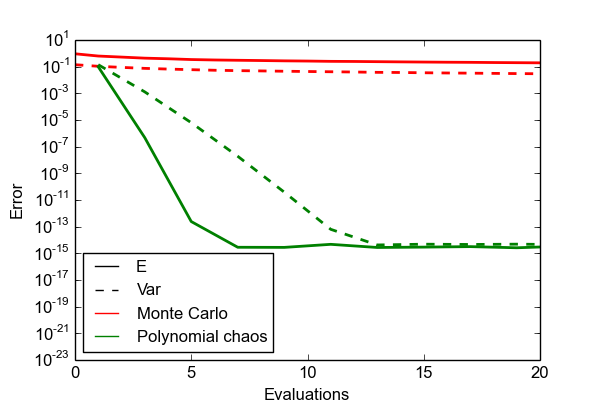
\includegraphics[width=0.85\textwidth]{Convergence_repeat.png}
 \end{figure}

\end{frame}



\begin{frame}
 \frametitle{The pseudo spectral approach: how I stopped worrying and learned to calculate the fourier coefficients}

 \begin{align*}
 c_i(x) &= \frac{\langle P_i,u(x,q)\rangle}{\norm{P_i}^2}\\
\onslide<2-> {&=\frac{1}{\norm{P_i}^2} \int P_i(q)u(x,q)f(q)dq} \onslide<3-> {\approx\\
   \hat{c}_i(x) &= \sum P_i(q_k)f(q_k)\omega_k}  
\end{align*}
\onslide<4->
\begin{itemize}
 \item $q_k$ - quadrature nodes
\item $\omega_k$ - quadrature weights

\end{itemize}

 \end{frame}
 
\begin{chaospy}{Repetition: 2D code}

 \begin{lstlisting}[language=python]
def u(x,a, I):
  return I*np.exp(-a*x)
|\pause| 
a = cp.Uniform(0, 0.1); I = cp.Uniform(8, 10)
dist = cp.J(a,I)|\pause|
x = np.linspace(0, 10, 100)
m = 2
|\pause| 
P = cp.orth_ttr(m, dist)|\pause|
nodes, weights = cp.generate_quadrature(m+1, dist,
                                        rule="G")|\pause|
i1,i2 = np.mgrid[:len(weights), :100]|\pause|
solves = u(x[i2],nodes[0][i1],nodes[1][i1])|\pause|
u_hat = cp.fit_quadrature(P, nodes, weights,
                          solves)
\end{lstlisting}
\end{chaospy}

\begin{frame}
 \frametitle{Quadrature rule, $\Pi$}
 \begin{table}
  \begin{tabular}{lcccccccc}
    $\Pi_0$& &&& $\bullet$& &&&  \\\hline
   $\Pi_1$ &&&$\bullet$& &$\bullet$&&& \\\hline
   $\Pi_2$ &&$\bullet$&&$\bullet$ &&$\bullet$&& \\
   \end{tabular}
\end{table}  
  
 Examples:
  \[\Pi_{11} = \begin{array}{cccc}
                 \bullet & & \bullet\\
                 &&\\
                 \bullet & & \bullet
                 \end{array}
\]
 \[ \Pi_{20} = \begin{array}{ccccc}
           \bullet & & \bullet & & \bullet
          \end{array}, \qquad \Pi_{12} = \begin{array}{cccc}
					\bullet&&\bullet\\\\
					\bullet&&\bullet\\\\
					\bullet&&\bullet
                                        \end{array}
 \]
 \end{frame}



\begin{frame}
 \frametitle{Plot of the nodes for the 2D problem, $\Pi_{44}$}
 \begin{figure}
  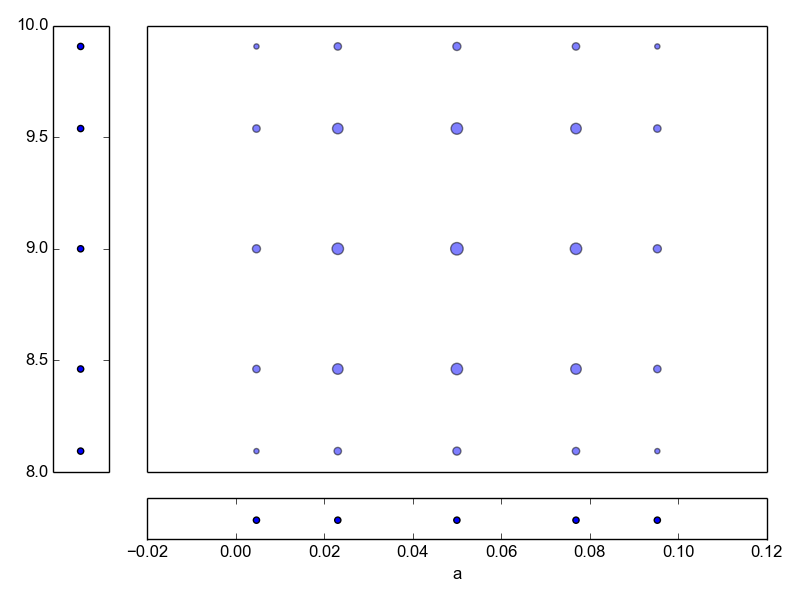
\includegraphics[width=0.85\textwidth]{nodes.png}
 \end{figure}
\end{frame}


\begin{frame}
 \frametitle{The number of nodes goes as, $k = (N+1)^D$}
 \begin{figure}
  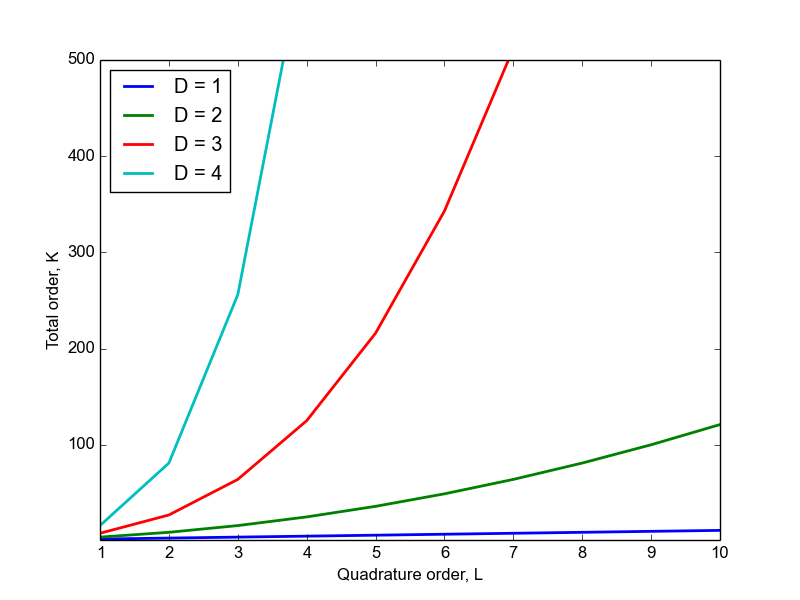
\includegraphics[width=0.85\textwidth]{dimensionality_nodes.png}
 \end{figure}
\end{frame}

\begin{frame}
 \frametitle{Solution: choose a smaller set of points that approximates the space, Smolyak sparse grids}

Full tensor basis:
\begin{table}
 \begin{tabular}{|c|c|c|}\hline
 $y^2$&$y^2x$&$y^2x^2$\\\hline
 $y$&$yx$&$yx^2$\\\hline
 $1$&$x$&$x^2$\\\hline
 \end{tabular}
\end{table}
\pause
Smolyak sparse grid:
 \begin{figure}
  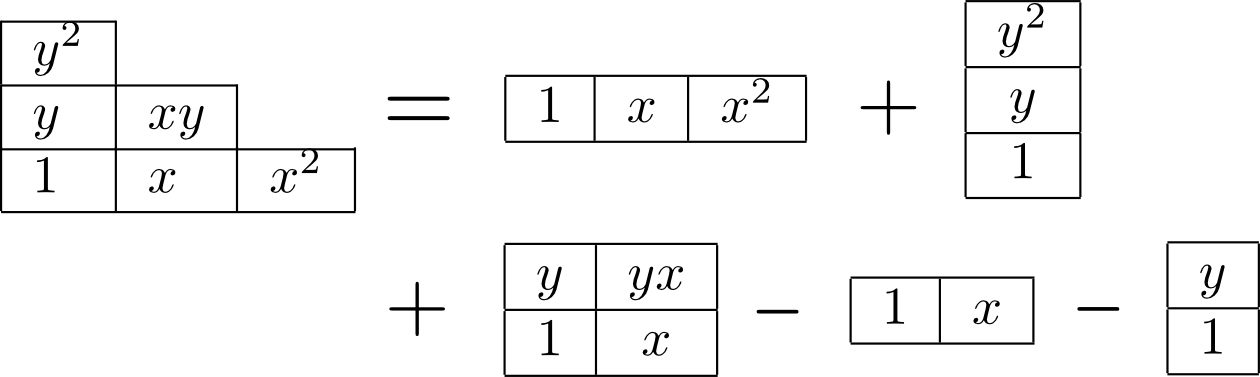
\includegraphics[width=0.9\textwidth]{smolyak2.png}
 \end{figure}
\[\Pi_{20} + \Pi_{11} + \Pi_{02} - \Pi_{10} - \Pi_{01}\]
\end{frame}

\begin{frame}
 \frametitle{Smolyak sparse grid, nodes}


 \begin{figure}
  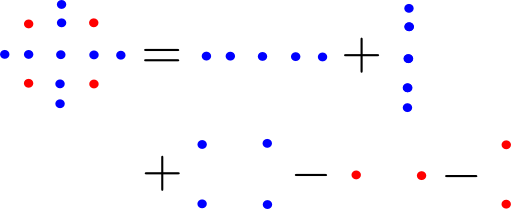
\includegraphics[width=\textwidth]{smolyak.png}
 \end{figure}

\end{frame}


\begin{frame}[fragile]
 \frametitle{Plot of the nodes for a 2D problem using a sparse grid}
 \begin{lstlisting}[language=python]
  nodes, weights = 
   cp.generate_quadrature(k, dist, rule="G",
                          sparse=True)
 \end{lstlisting}

 \pause
 \begin{figure}
  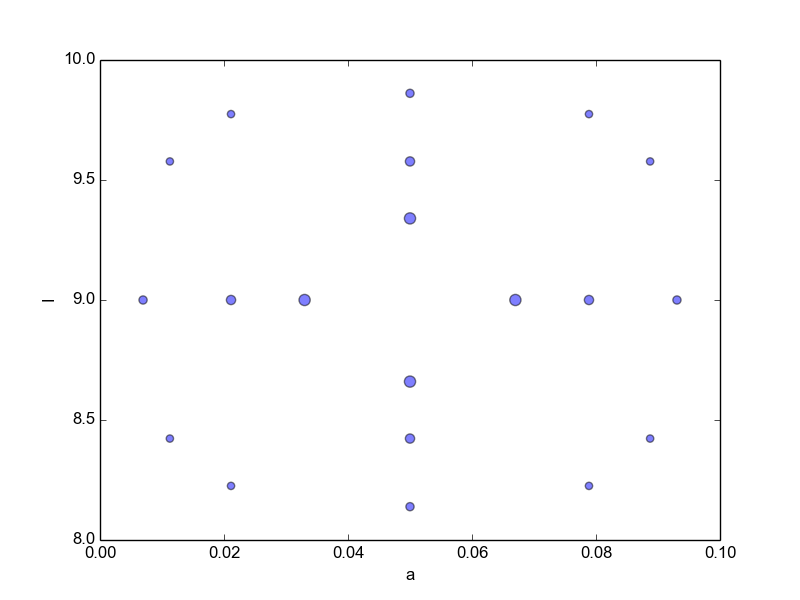
\includegraphics[width=0.6\textwidth]{nodes_sparse.png}
 \end{figure}
\end{frame}
 
\begin{frame} 
  \begin{figure}
  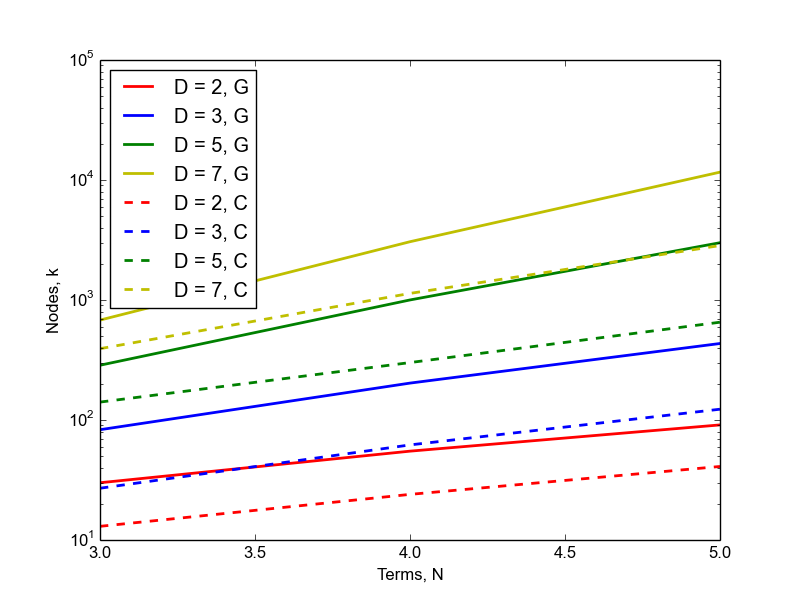
\includegraphics[width=0.85\textwidth]{dimensionality_nodes_sparse.png}
 \end{figure}
 \end{frame}
 
 \begin{frame}
  \frametitle{Nested sparse grids}
  
 Clenshaw-Curtis:\\
 cp.generate\_quadrature(k, dist, rule="C",growth=False)
  \begin{table}
  \begin{tabular}{lcccccccc}
    $\Pi_0$& &&& $\bullet$& &&&  \\\hline
   $\Pi_1$ &&&$\bullet$& &$\bullet$&&& \\\hline
   $\Pi_2$ &&$\bullet$&&$\bullet$ &&$\bullet$&& \\
   \end{tabular}
  \end{table}
  
  
  Nested Clenshaw-Curtis:\\
  cp.generate\_quadrature(k, dist, rule="C",growth=True)
  \begin{table}
  \begin{tabular}{lcccccccc}
    $\Pi_0$& &&& $\bullet$& &&&  \\\hline
   $\Pi_1$ &&$\bullet$&& $\bullet$&&$\bullet$ && \\\hline
   $\Pi_2$ &$\bullet$&$\bullet$&$\bullet$& $\bullet$&$\bullet$&$\bullet$ &$\bullet$& \\
   \end{tabular}
  \end{table}
 
  \end{frame}

\begin{frame}
 \frametitle{Nested smolyak sparse grid, nodes}


 \begin{figure}
  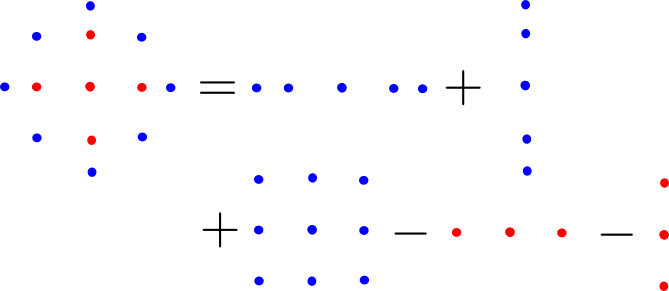
\includegraphics[width=\textwidth]{smolyak_nested.png}
 \end{figure}

\end{frame}

\begin{frame}
 \frametitle{Nested smolyak sparse grid, nodes}
 \begin{figure}
  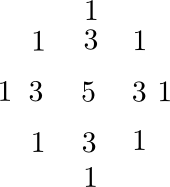
\includegraphics[width=0.5\textwidth]{smolyak_nested_nr.png}
 \end{figure}

\end{frame}

 
 \begin{frame}
 \frametitle{Clenshaw-Curtis quadrature vs Gaussian quadrature}
 \begin{figure}        
 \begin{subfigure}[b]{0.5\textwidth}
                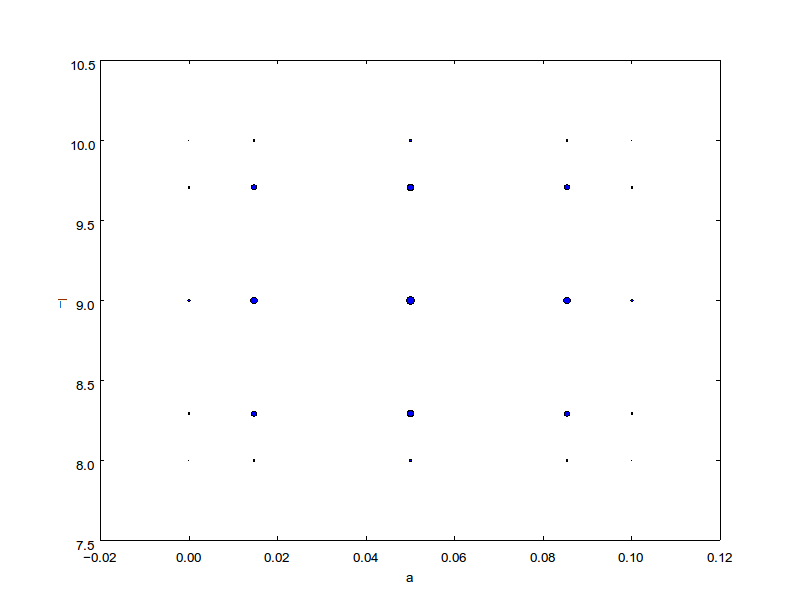
\includegraphics[width=\textwidth]{nodes_C.png}
                \caption{Clenshaw-Curtis quadrature}
        \end{subfigure}%        
 \begin{subfigure}[b]{0.5\textwidth}
                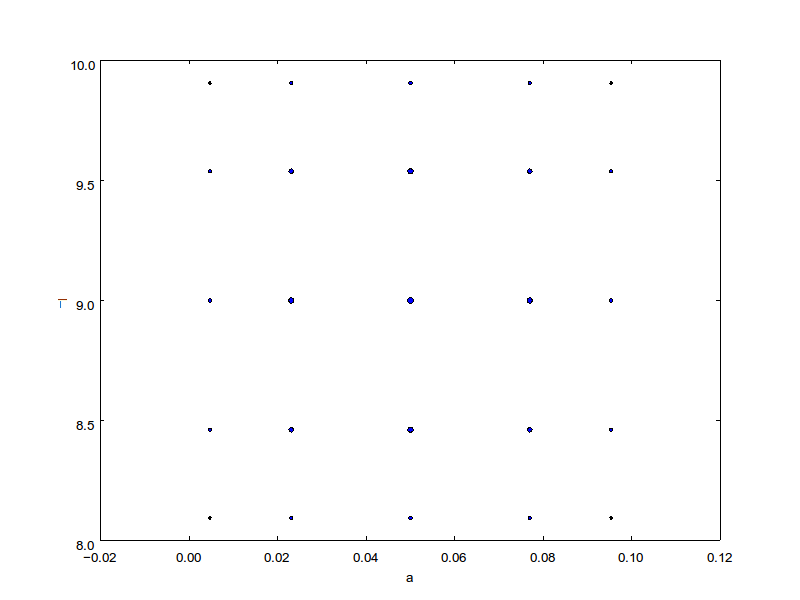
\includegraphics[width=\textwidth]{nodes_G.png}
                \caption{Gaussian quadrature}
        \end{subfigure}
        \end{figure}
\end{frame}
 
 
 \begin{frame}
  \frametitle{Number of nodes needed}
  \begin{itemize}
   \item $L$ is the number of nodes along one axis
  \end{itemize}

 \begin{figure}
  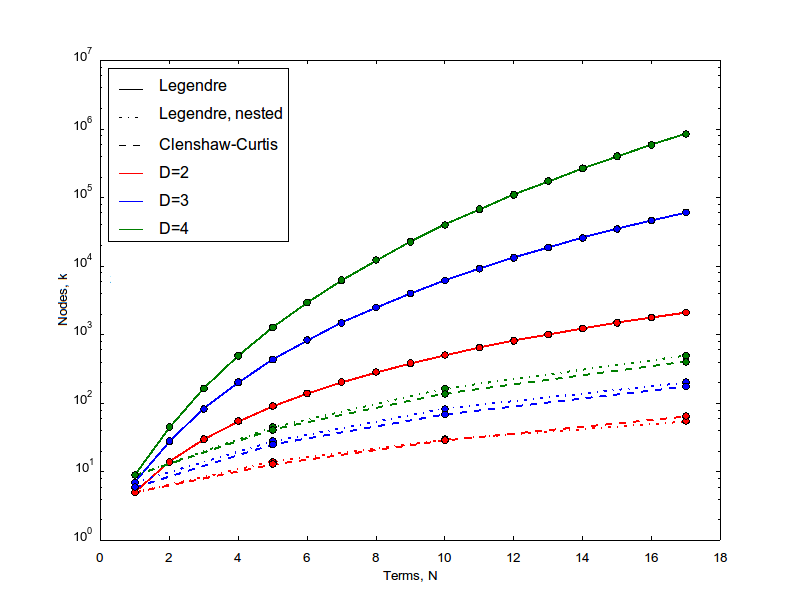
\includegraphics[width=0.85\textwidth]{dimensionality_nodes_nested.png}
 \end{figure}
 \end{frame}

  
  \begin{frame}
   \frametitle{Mapping between order, M and number of nodes , L}
   For nested Clenshaw-Curtis
   \begin{figure}
    \includegraphics<1>[width=0.85\textwidth]{LvsM1.png}
    \includegraphics<2>[width=0.85\textwidth]{LvsM.png}
   \end{figure}

   
  %\begin{tabular}{lccccccccccc}
  % Order, M & 0 & 1 & 2 & 3 & 4 & 5 & 6 & 7 & 8 \\\\
  % Quad  & 1 & 4 & 9 & 16 & 25 & 36 & 49 & 64 & 81 \\\\
  % Poly  & 1 & 3 & 6 & 10 & 15 & 21 & 28 & 37 & 37
  %\end{tabular}

  \end{frame}

  
  
  \begin{frame}
 \frametitle{Difference }
 \begin{figure}        
 \begin{subfigure}[b]{0.5\textwidth}
                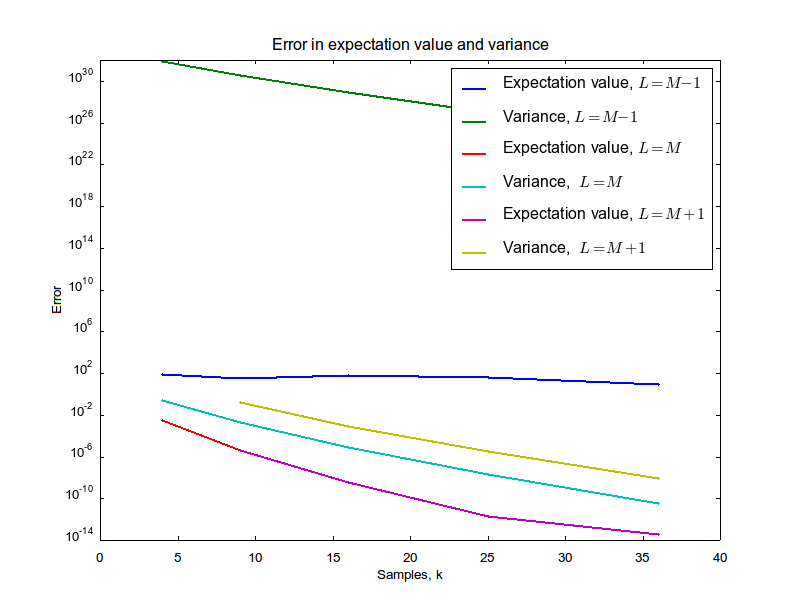
\includegraphics[width=\textwidth]{convergence_2D_L.png}
                \caption{$L=M-1$, $L=M$, $L=M+1$}
        \end{subfigure}%        
 \begin{subfigure}[b]{0.5\textwidth}
                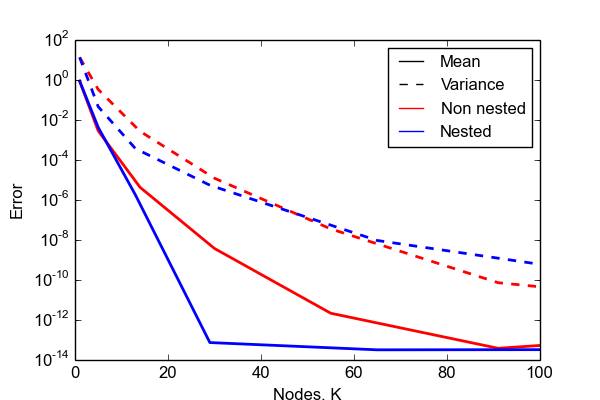
\includegraphics[width=\textwidth]{convergence_2D_L_sparse.png}
                \caption{Sparse grid: $L=M-1$, $L=M$}
        \end{subfigure}
        \end{figure}
\end{frame}
  
  
  
 \begin{frame}
  \frametitle{Definition of Gaussian quadrature}
  \begin{align*}
   \int W(q)u(x,q)dq &\approx \sum_k \omega_k u(x,q_k)\\
   \intertext{for a weighting function $W(q)$}
   \uncover<2-> {\int f(q)u(x,q)dq \approx \sum_k \omega_k u(x,q_k)}
    \end{align*}
   \end{frame}

 
  \begin{frame}
 \frametitle{Nodes for different probability distributions}
 \begin{figure}        
 \begin{subfigure}[b]{0.37\textwidth}
                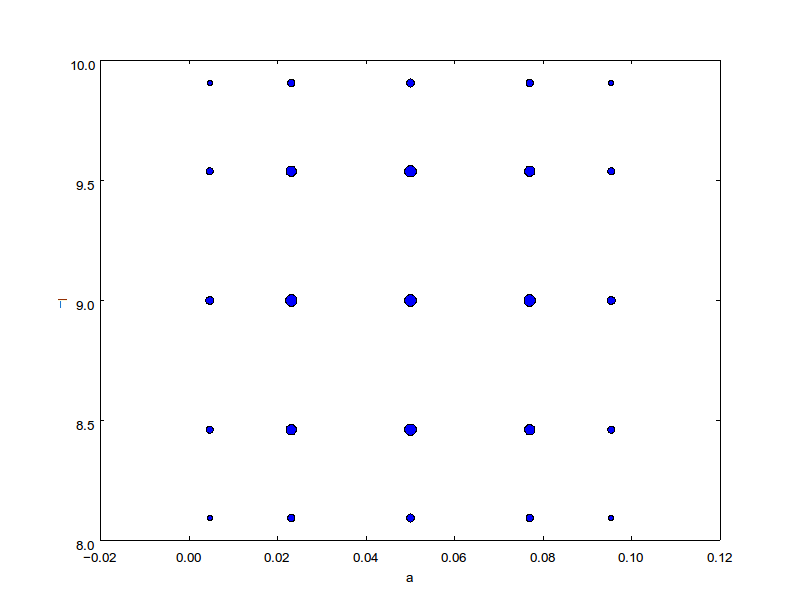
\includegraphics[width=\textwidth]{nodes_uniform.png}
                \caption{Uniform}
        \end{subfigure}%        
 \begin{subfigure}[b]{0.37\textwidth}
                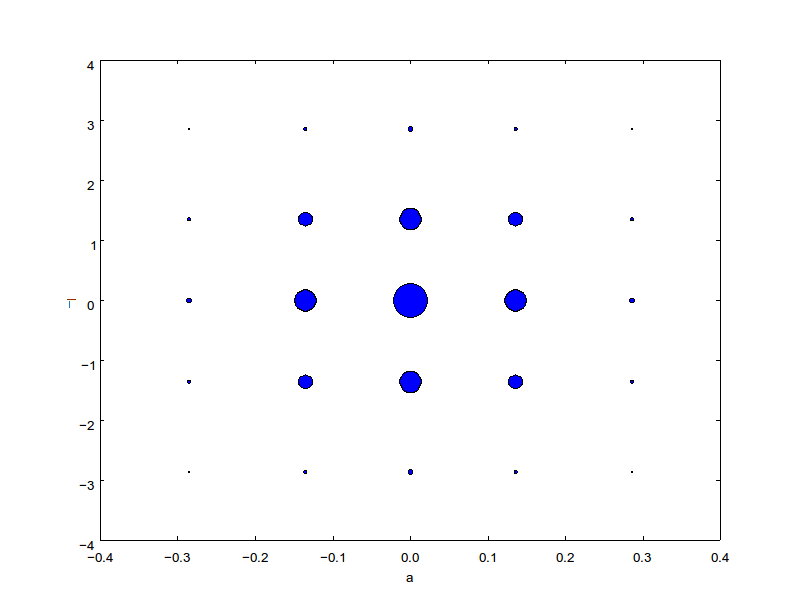
\includegraphics[width=\textwidth]{nodes_normal.png}
                \caption{Normal}
        \end{subfigure}
 \begin{subfigure}[b]{0.37\textwidth}
                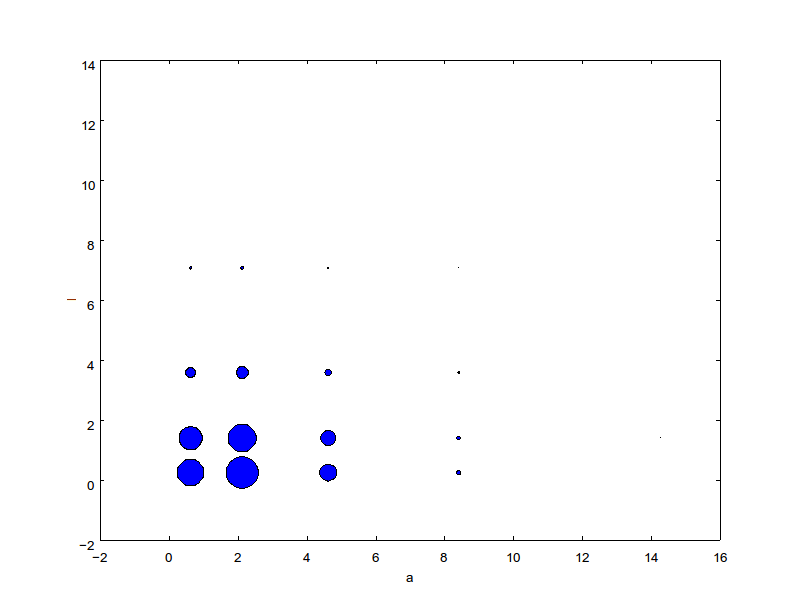
\includegraphics[width=\textwidth]{nodes_gamma.png}
                \caption{Gamma}
        \end{subfigure}%        
 \begin{subfigure}[b]{0.37\textwidth}
                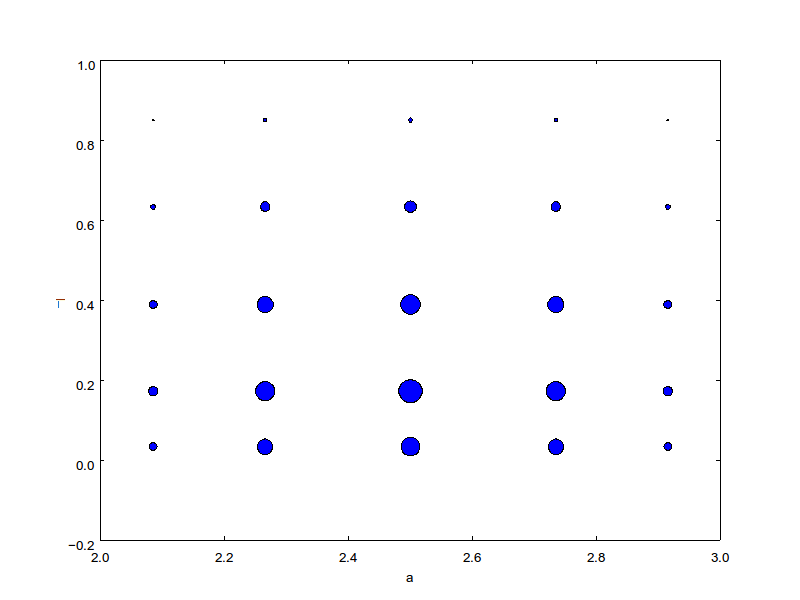
\includegraphics[width=\textwidth]{nodes_beta.png}
                \caption{Beta}
        \end{subfigure}
        \end{figure}
               
\end{frame}
 
 
 \begin{frame}
  \frametitle{Convergence for Gaussian quadrature vs Legendre}
  \begin{figure}
   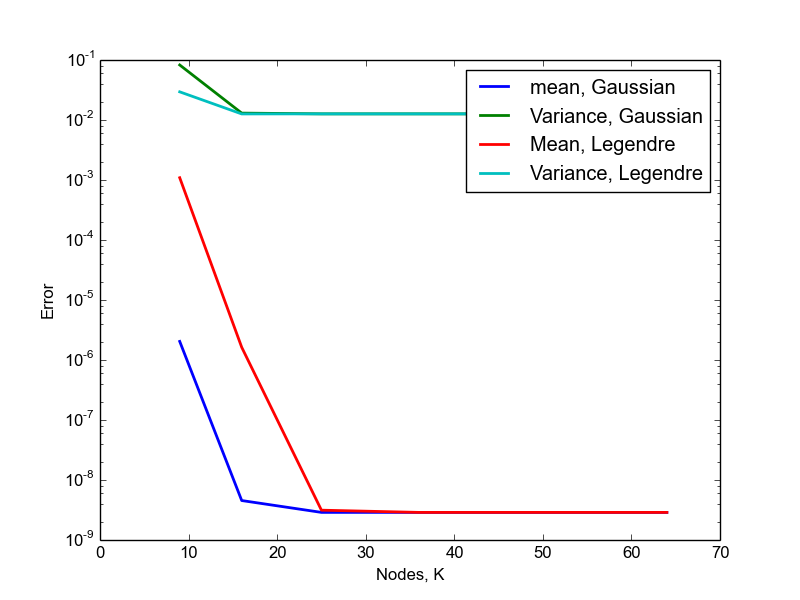
\includegraphics[width=0.85\textwidth]{convergence_GvsL.png}
  \end{figure}

 \end{frame}

 
 \begin{frame}
  \frametitle{Point collocation}
  \begin{center}
 \begin{tabular}{cc}
   $\vec{C} = \left[
  \begin{matrix}
  C_0  \\
  \vdots \\
  C_N 
 \end{matrix}\right]$
 & $\vec{P} = \left[
  \begin{matrix}
  P_0(q_0) & \dots & P_N(q_0)  \\
  \vdots & & \vdots \\
  P_0(q_k) & \dots& P_N(q_k) 
 \end{matrix}\right]$
 \end{tabular}
\end{center}

\[\vec{U} = \left[
  \begin{matrix}
  u(x,q_0)  \\
  \vdots \\
  u(x,q_k) 
 \end{matrix}\right]\]
 
 \end{frame}

 
 
\begin{frame}
 \frametitle{Least square minimization}
 \[\vec{P}\cdot \vec{C}= \vec{U}\]
 \[\hat{c} = (\vec{P}^T\vec{P})^{-1}\vec{P}^T\vec{U}\]
\end{frame}


\begin{frame}
 \frametitle{Convergence using least square minimization}
 \begin{figure}
  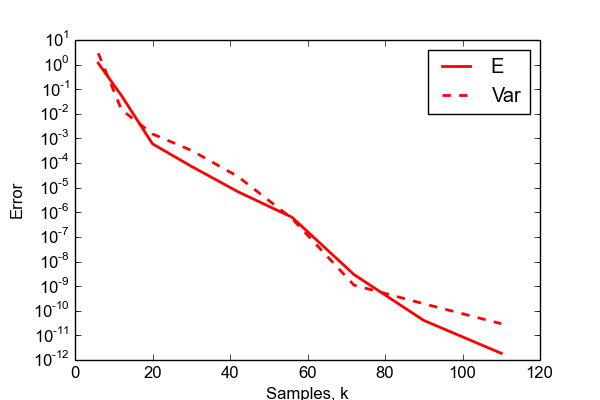
\includegraphics[width=0.85\textwidth]{convergence_collocation.png}
 \end{figure}
\end{frame}


\begin{chaospy}{Code for least square minimization}
 \begin{lstlisting}[language=python]
def u(x, a, I):
  return I*np.exp(-a*x)
 |\pause|
a = cp.Uniform(0, 0.1)
I = cp.Uniform(8, 10)
dist = cp.J(a,I)
|\pause|
x = np.linspace(0, 10, 100)
 |\pause|
P = cp.orth_ttr(n, dist) |\pause|
nodes = dist.sample(2*len(P), "H") |\pause|
solves = [u(T, s[0], s[1]) for s in nodes.T] |\pause|
U_hat = cp.fit_regression(P, nodes, solves,
                          rule="LS")
 \end{lstlisting}

\end{chaospy}


\begin{frame}
 \frametitle{Sampling scheme}
 \begin{figure}
  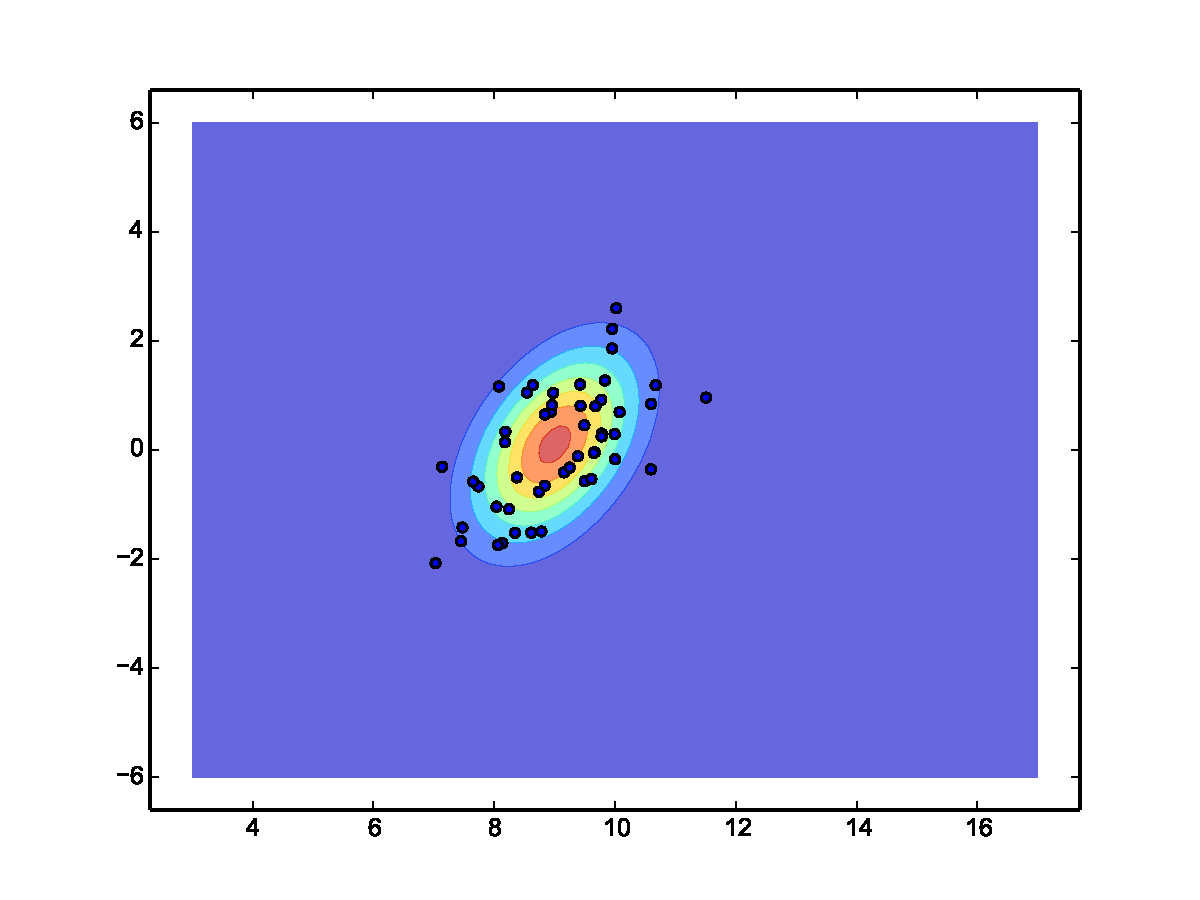
\includegraphics[width=0.85\textwidth]{sampling.pdf}
 \end{figure}
 
\end{frame}

  \begin{frame}
 \frametitle{Different sampling schemes}
 \begin{figure}        
 \begin{subfigure}[b]{0.5\textwidth}
                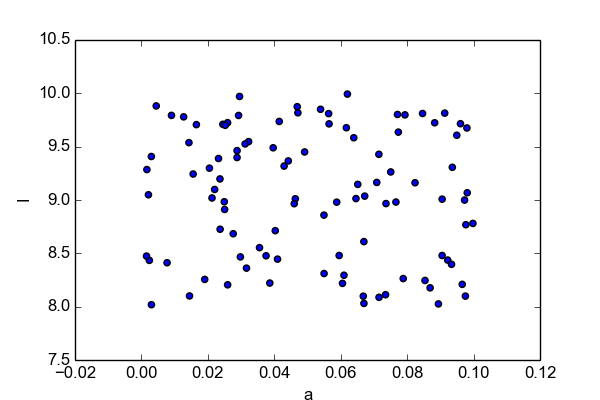
\includegraphics[width=\textwidth]{samples.png}
                \caption{Sobol sampling, default: \\                
                nodes = dist.sample(100)}
        \end{subfigure}%        
 \begin{subfigure}[b]{0.5\textwidth}
                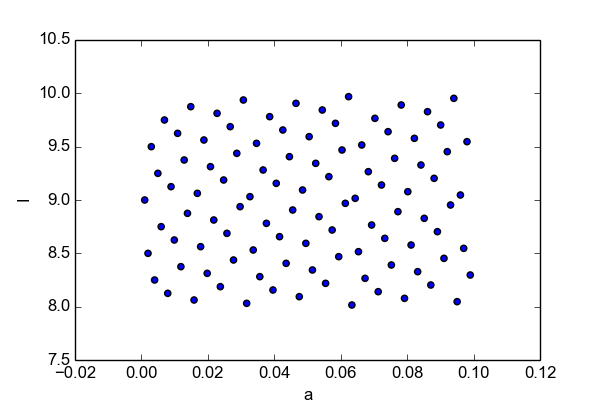
\includegraphics[width=\textwidth]{samples_M.png}
                \caption{Hammersley sampling: \\                
                nodes = dist.sample(100, "M")}
        \end{subfigure}
        \end{figure}
\end{frame}
  


\begin{frame}
 \frametitle{Convergence using different sampling schemes}
  \begin{figure}
  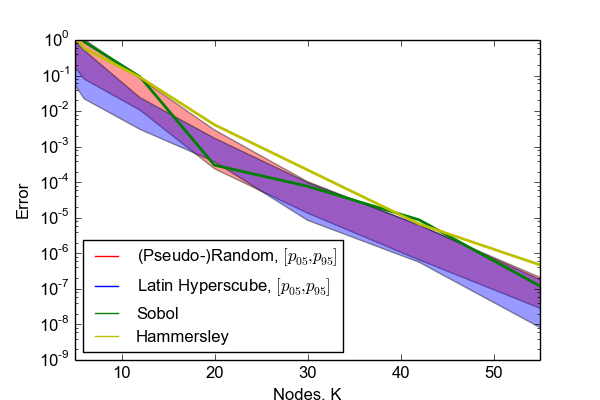
\includegraphics[width=0.85\textwidth]{convergence_collocation_compare.png}
 \end{figure}
\end{frame}



\begin{chaospy}{Analysis of the 2D problem}
 \begin{lstlisting}[language=python]
def u(x,a, I):
  return I*np.exp(-a*x)
|\pause|
a = cp.Uniform(0, 0.1)
I = cp.Uniform(8, 10)
dist = cp.J(a,I)
|\pause|
x = np.linspace(0, 10, 100); M = 5
|\pause|
P, norm = cp.orth_ttr(M, dist, retall=True) |\pause|
nodes, weights = cp.generate_quadrature(M+1, dist,
                                        rule="G")|\pause|
solves = [u(x, s[0], s[1]) for s in nodes.T] |\pause|
U_hat, c = cp.fit_quadrature(P, nodes, weights,
                             solves, retall=True)
 \end{lstlisting}
\end{chaospy}


\begin{chaospy}{Analysis of the 2D problem continued}
 \begin{lstlisting}[language=python]
E_1 =  cp.E(U_hat,dist)
E_2 = c[0]
|\pause|
Var_1 = cp.E(U_hat,dist)
Var_2 = np.sum(norm[1:]*c[1:].T**2,1)
|\pause|
s = dist.sample(10**6)
u_mc = U_hat(*s)
|\pause|
E_3 = np.mean(u_mc,1)
Var_3 = np.var(u_mc,1)
\end{lstlisting}
\end{chaospy}

\begin{frame}
 \frametitle{Expectation value}
   \begin{figure}
    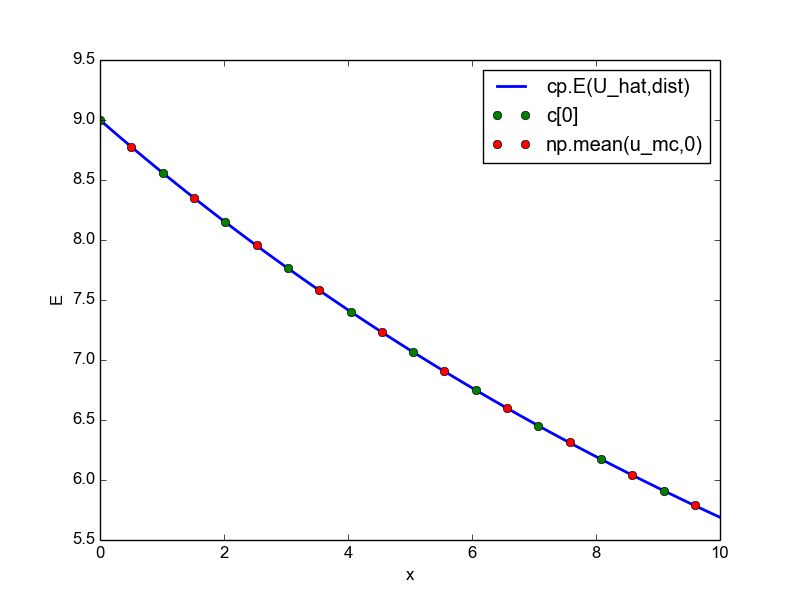
\includegraphics[width=0.85\textwidth]{E.png}
   \end{figure}
\end{frame}

\begin{frame}
 \frametitle{Variance}
   \begin{figure}
    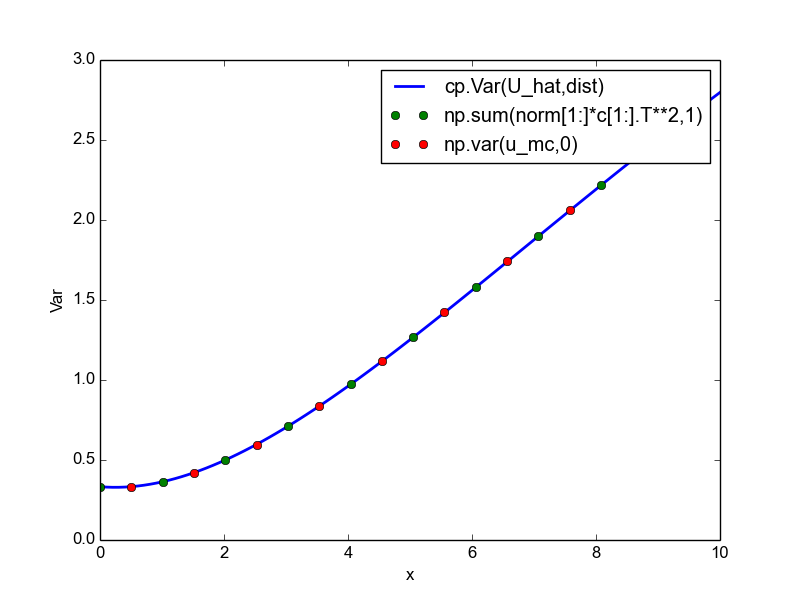
\includegraphics[width=0.85\textwidth]{Var.png}
   \end{figure}
\end{frame}

\begin{frame}[fragile]
 \frametitle{Variance based sensitivity}
 \begin{align*}
  S_{T_i} &= \frac{E(Var(u | dist \backslash d_i ))}{Var(u)}\\
\onslide<2->{&= \frac{E(E(u^2 | dist \backslash d_i ) - E((u | dist \backslash d_i )^2))}{Var(u)}}
\end{align*} 
\onslide<3->
Code:
 \begin{lstlisting}[language=python]
  S_Ti = cp.Sens_t(U_hat, dist)
 \end{lstlisting}
\end{frame}


\begin{frame}
 \frametitle{Variance based sensitivity}
  \begin{figure}
  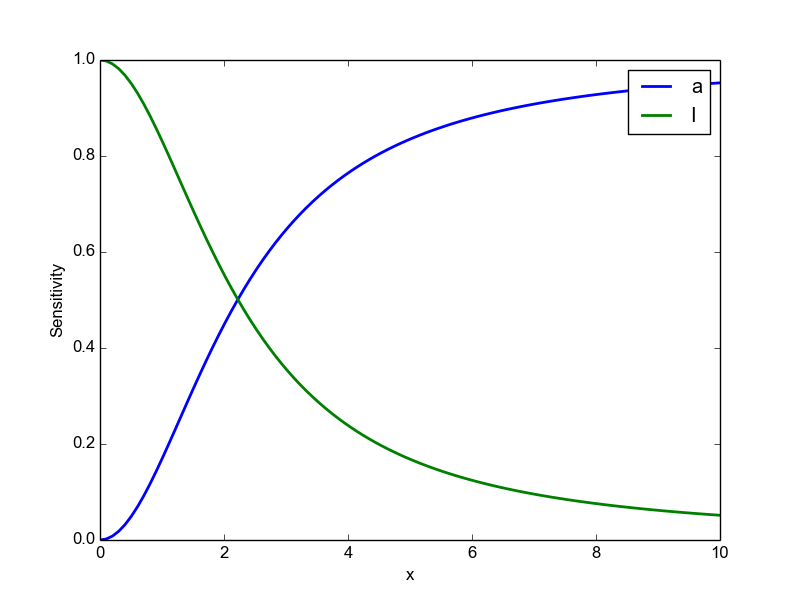
\includegraphics[width=0.85\textwidth]{sens.png}
 \end{figure}
\end{frame}



\begin{chaospy}{Calculate confidence interval}
  \begin{lstlisting}[language=python]
p_10 = np.percentile(u_mc,10,1)
p_90 = np.percentile(u_mc,90,1)
 \end{lstlisting}
\end{chaospy}

\begin{frame}[fragile]
 \frametitle{Confidence interval}
  \begin{figure}
  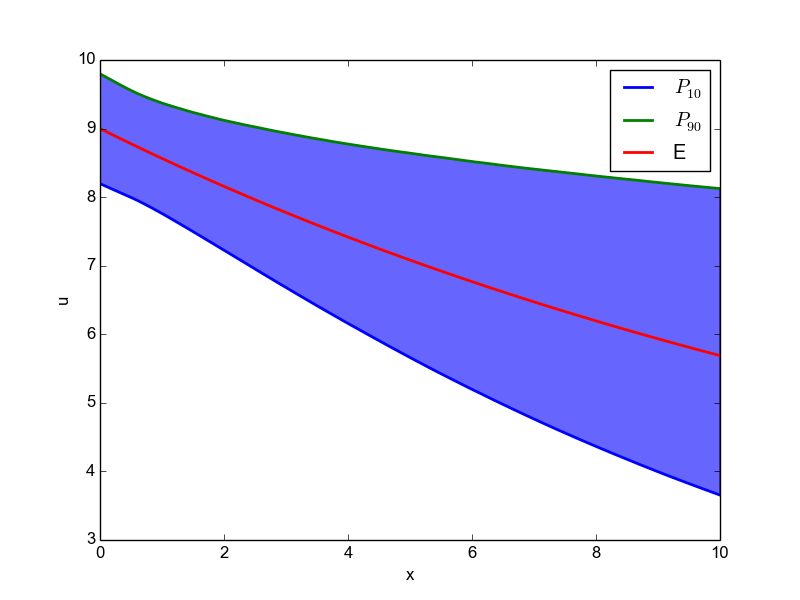
\includegraphics[width=0.85\textwidth]{percentiles.png}
 \end{figure}
 
\end{frame}


\begin{chaospy}{Summary}
 \begin{lstlisting}[language=python]
def u(x,a, I):
  return I*np.exp(-a*x)
|\pause|
a = cp.Uniform(0, 0.1)
I = cp.Uniform(8, 10)
dist = cp.J(a,I)
|\pause|
x = np.linspace(0, 10, 100); M = 5
 \end{lstlisting}

\end{chaospy}

\begin{chaospy}{Summary continued}
\begin{lstlisting}[language=python]
P = cp.orth_ttr(M, dist) |\pause|
nodes, weights = cp.generate_quadrature(M+1, dist,
                                        rule="G")|\pause|
solves = [u(x, s[0], s[1]) for s in nodes.T] |\pause|

U_hat= cp.fit_quadrature(P, nodes, weights,
                         solves)|\pause|
                         
mean = cp.E(U_hat, dist)|\pause|
var = cp.Var(U_hat, dist)
\end{lstlisting}

\end{chaospy}



\end{document}
